\chapter{Третья глава. Программная реализация алгоритма}
\label{cha:ch_3}
\section{Общая схема вычислений}

\par
В рассмотренных далее примерах рассматривалась вероятностная реализация алгоритмов CFR и MCCFR. При использовании метода MCCFR значения случайных событий генерируются перед началом каждой обучающей итерации. Данный подход позволяет сократить обьем памяти и ускорить вычисления в некоторых случаях\cite{MCCFR}.
При реализации примеров были выделены следующие компоненты:
\begin{itemize}
	\item описание правил игры (зависит от настроек);
	\item модуль с реализацией алгоритма относительно определенных правил.
\end{itemize}
\par
Настройки игры, например, по возможности могут включать число игроков, параметры выплат и т.п.
\par
Правила игры включают структуру игрового дерева, механизм распределения событий и функцию выплат. Игровое дерево строится с применением узлов -- обьектов с информацией о историии игры, о игроке и о возможных действиях.
\par
Итерации алгоритма проходят рекурсивно, начиная с вершины дерева. В ходе одной итерации t + 1 происходит следующее:
\begin{itemize}
\item расчет стратегий $q^{t + 1}$ используя $t$ контрафактические сожаления(1.8);
\item расчет $t + 1$ слагаемого контрафактических сожалений;
\item обновление сумм контрафактических сожалений (1.7).
\end{itemize}
\par
Сам расчет итераций CFR происходит в выделенном модуле, на основе, определенных для каждого конкретного случая, правил игры. Работа алгоритма начинается с создания игрового дерева. Далее происходит расчет заданного числа итераций. После любой итерации можно получить стратегии игроков, которые представляют из себя приближенное коррелированное равновесие.

\section{Разоблачение совместного преступления}

Рассмотрим несколько частных случаев задачи разоблачения совместного преступления. В соответствии с определением 1.1, опишем игровые истории и информационные наборы игроков.
\begin{align*}
	A = \{\text{Предложить взятку}, \text{Не предлагать взятку}, \text{Принять взятку}, \\ \text{Отклонить взятку}, \text{Провести проверку}, \text{Не проводить проверку} \}
\end{align*}
Также определим перечень всех досупных игровых историй, включая терминальные:
\begin{align*}
hB = & \{\text{Предложить взятку}\} \\
hBT = & \{\text{Предложить взятку}, \text{Принять взятку}\} \\
zBTC = & \{\text{Предложить взятку}, \text{Принять взятку}, \text{Провести проверку}\} \\
zBTnC = & \{\text{ Предложить взятку}, \text{Принять взятку}, \text{Не проводить проверку}\} \\
hBnT = & \{ \text{Предложить взятку}, \text{Отклонить взятку} \} \\
zBnTC = & \{\text{ Предложить взятку}, \text{Отклонить взятку}, \text{Провести проверку}\} \\
zBnTnC = & \{\text{ Предложить взятку}, \text{Отклонить взятку}, \text{Не проводить проверку}\} \\
hnB = & \{\text{ Не предлагать взятку}\} \\
znBC = & \{\text{ Не предлагать взятку}, \text{Провести проверку}\} \\
znBnC = & \{\text{ Не предлагать взятку}, \text{Не проводить проверку} \}
\end{align*}
\begin{equation*}
	H = \{\emptyset, hB, hBT, zBTC, zBTnC, hBnT, zBnTC, zBNCnC, hnB, znBC, znBnC\}
\end{equation*}
\begin{equation*}
Z = \{zBTC, zBTnC, zBnTC, zBnTnC, znBC, znBnC\}
\end{equation*}
\par
Будем рассматривать множество $N$, состоящее из трех игроков: клиент, чиновник и инспектор
\begin{equation*}
N = \{0, 1, 2\}
\end{equation*}
Далее, определим информационные состояния игроков. В данном случае информационные наборы каждого игрока состоят из одного информационного состояния
\begin{align*}
\mathcal{I}_0 = & \{\{\emptyset\}\} \\
\mathcal{I}_1 = & \{\{hB\}\} \\
\mathcal{I}_2 = & \{\{hBT, hBnT, hnB\}\}
\end{align*}
\par
Данное определение информационных состояний позволяет сопоставить игроков и различные игровые истории и таким образом определить функцию $P$.

$$P(h0) = 0$$
$$P(hB)=1$$
$$P(hBT)=P(hBnT)=P(hnB)=2$$

Наконец, определим следующие терминальные выплаты для игроков из $N$ на множестве $Z$. В таблице \ref{tbl:u1} указано значение функции $u_i(z)$, для игрока $i \in N$ и терминальной истории $z \in Z$.

\begin{table}[H]
	\centering
	\begin{tabular}[t]{|c|c|c|c|c|c|c|}
		\hline
		$u$ &	$zBTC$ & $zBTnC$ &	$zBnTC$ & $zBnTnC$ & $znBC$ & $znBnC$ \\
		\hline
		$0$	&$v-b-p_L-p_H$&	$v-b$&	$-p_L$&	$0$&	$0$ &	$0$ \\
		\hline
		$1$&	$b-q$&	$b$&	$r$&	$r$&	$0$&	$0$ \\
		\hline
		$2$&	$x+\Delta x$&	$x$&	$y+\Delta y$&	$y$&	$z$&	$z+\Delta z$ \\
		
		\hline
	\end{tabular}
	\caption{\centering Значения функции выплат $u$}
	\label{tbl:u1}
\end{table}

Проведем расчеты для некоторых значений параметров. Рассмотрим набор параметров из таблицы \ref{tbl:s1_1} и проведем расчет равновесия для данного случая

\begin{table}[H]
	\centering
	\begin{tabular}[t]{|c|c|c|c|c|c|c|c|c|c|c|c|}
		\hline
		$v$ &	$b$ & $p_L$ &	$p_H$ & $q$ & $r$ & $\Delta x$ & $x$ & $\Delta y$ & $y$ & $\Delta z$ & $z$ \\
		\hline
		6 &	4 & 3 &	3 & 5 & 1 & 6 & -3 & 4 & -2 & 2 & -1 \\
		\hline
	\end{tabular}
\caption{\centering Значения параметров для первого примера}
\label{tbl:s1_1}
\end{table}
\par
Учитывая параметры из таблицы \ref{tbl:s1_1} построим игровое дерево со случайным профилем стратегий. Схематичное изображение игрового дерева показано на рисунке \ref{fig:c3th11}.

\begin{figure}[h]
	\centering
	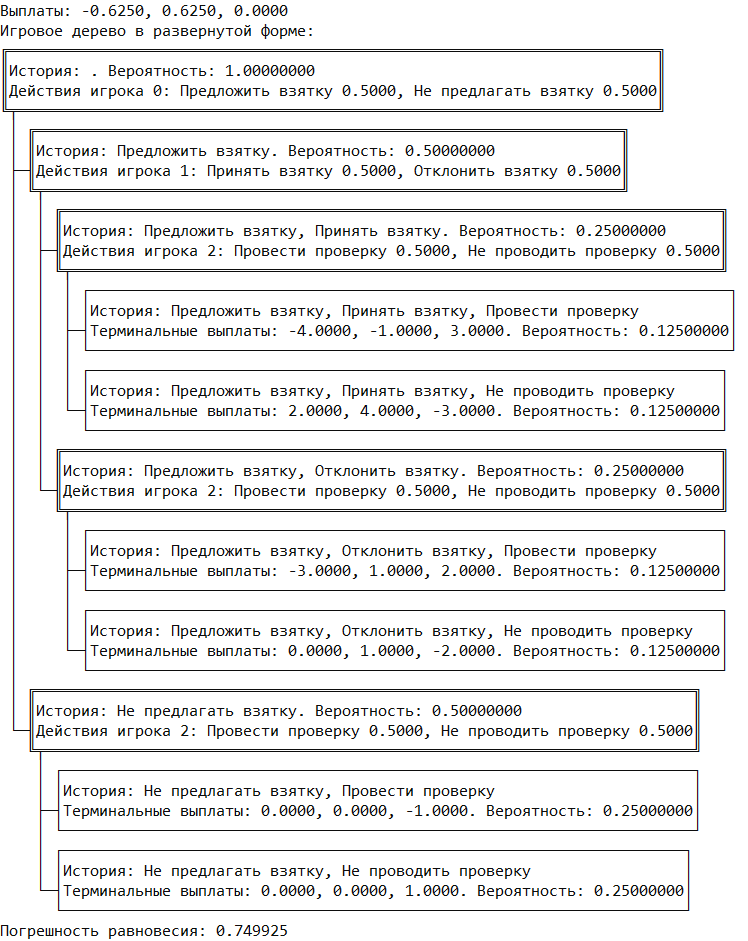
\includegraphics[width=0.9\linewidth]{inc/img/c3th11}
	\caption{Дерево игры с первой группой параметров. Случайные стратегии}
	\label{fig:c3th11}
\end{figure}

\par
На рисунке \ref{fig:c3th11} прямоугольными элементами отмечены все игровые истории, начиная с начала игры. Ребра между элементами обозначают возможные переходы между игровыми историями. Каждой нетерминальной игровой истории соответствует перечень доступных действий и стратегия их выбора. Терминальные истории сопровождаются информацией о выплатах игрокам. Для каждой истории указывается вероятность ее реализации. Расчетная эксплуатируемость данного профиля стратегий составляет примерно $0.75$. Для достижения этого значения инспектору достаточно проводить проверку с вероятностью $1.0$, изменив тем самым свой ожидаемый выигрыш с $0$ до $0.75$. Данный стратегический профиль достаточно далек от равновесия.
\par
Попробуем улучшить стратегический профиль. Проведем $T=10000$ обучающих итераций алгоритма на данном игровом дереве. Информация о обновленном стратегическом профиле представлена на рисунке \ref{fig:c3th12}.
\begin{figure}[h]
	\centering
	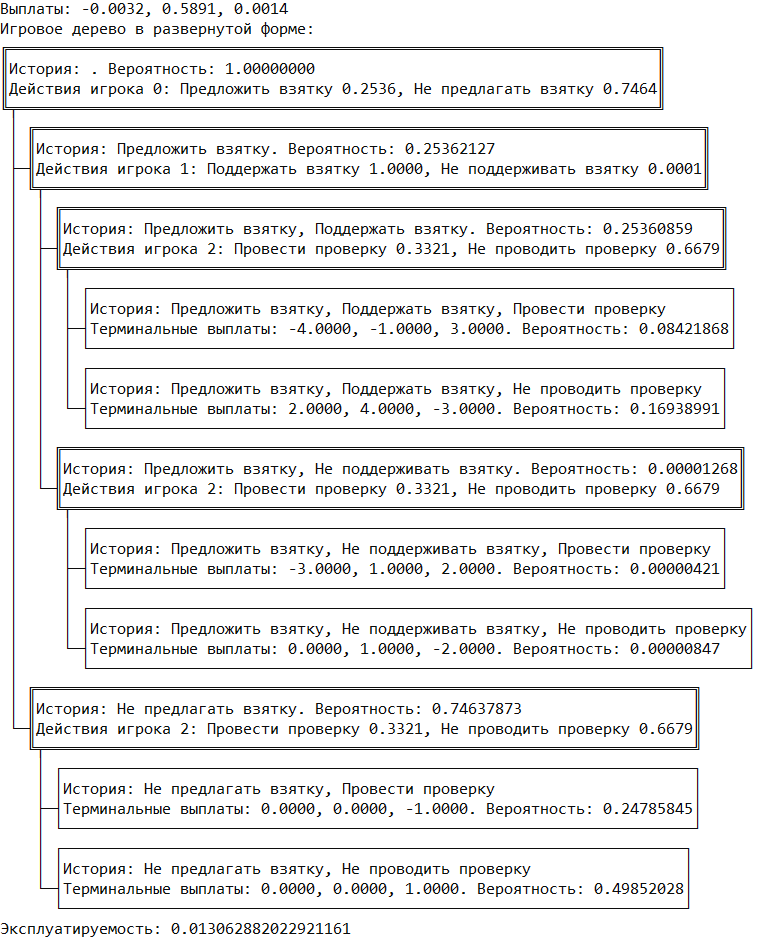
\includegraphics[width=0.9\linewidth]{inc/img/c3th12}
	\caption{Дерево игры с первой группой параметров. $T = 10000$}
	\label{fig:c3th12}
\end{figure}
\par
На рисунке \ref{fig:c3th12} отмечены выплаты, измененные стратегии игроков и измененные вероятности достижения различных игровых историй. Как можно заметить, эксплотируемость снизилась до порядка $0.01$, что сопоставимо с оценкой из теоремы \ref{CfrTStrategyExp}.
\par
Дальнейшее увеличение числа итераций приводит к снижению эксплуатируемости. График изменения расчетной эксплуатируемости для данного примера приведен на рисунке \ref{fig:c3e1}.

\begin{figure}[H]
	\centering
	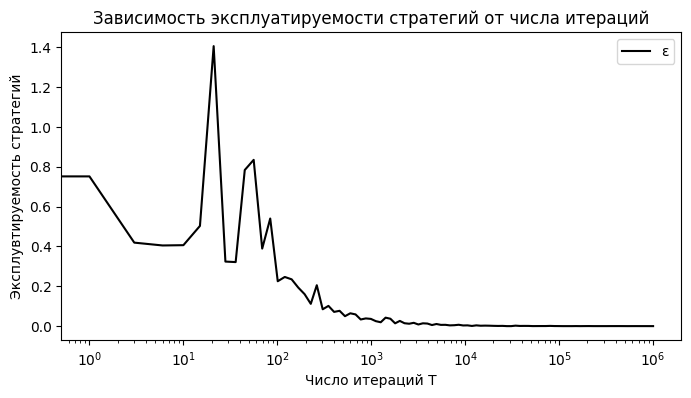
\includegraphics[width=0.8\linewidth]{inc/img/c3e1}
	\caption{Расчетная эксплуатируемость стратегий в зависимости от $T$}
	\label{fig:c3e1}
\end{figure}

\par
Рассмотрим другой набор параметров алгоритма (Таблица \ref{tbl:s1_2}).
\begin{table}[H]
	\centering
	\begin{tabular}[t]{|c|c|c|c|c|c|c|c|c|c|c|c|}
		\hline
		$v$ &	$b$ & $p_L$ &	$p_H$ & $q$ & $r$ & $\Delta x$ & $x$ & $\Delta y$ & $y$ & $\Delta z$ & $z$ \\
		\hline
		12 &	3 & 8 &	8 & 4 & 2 & 9 & 1 & 1 & 7 & 3 & 5 \\
		\hline
	\end{tabular}
	\caption{\centering Значения параметров для второго примера}
	\label{tbl:s1_2}
\end{table}
\par
Построим игровую модель и проведем $10000$ обучающих итераций. Полученный профиль стратегий представлен на рисунке \ref{fig:c3th21}.
\begin{figure}[H]
	\centering
	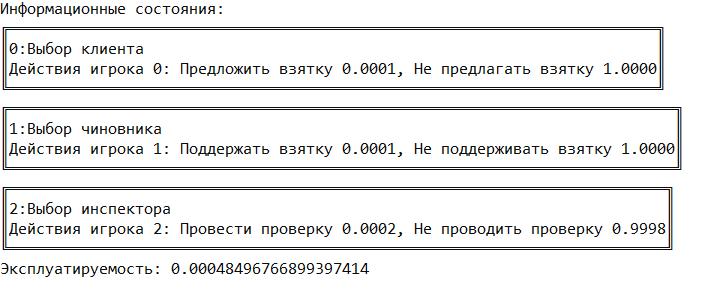
\includegraphics[width=0.8\linewidth]{inc/img/c3th21}
	\caption{Стратегии игроков для второго примера. $T=10000$}
	\label{fig:c3th21}
\end{figure}
\par
В результате мы получили профиль, который состоит из чистых стратегий. Хотя данное решение и является равновесием, оно маловероятно на практике по интуитивным соображениям. Так как алгоритм предоставляет единственное решение, имеет смысл наложить дополнительные ограничения на рассматриваемую задачу. Попробуем получить дополнительную информацию о данной игре. Для этого попробуем зафиксировать стратегию одного игрока и найти равновесие для двух оставшихся. Таким образом, найдем зависимости $\beta$ и $\gamma$ от $\alpha$, $\alpha$ и $\gamma$ от $\beta$ и зависимость $\alpha$ и $\beta$ от $\gamma$. Графики соответствующих зависимостей представлены на рисунках .

\begin{figure}[H]
	\centering
	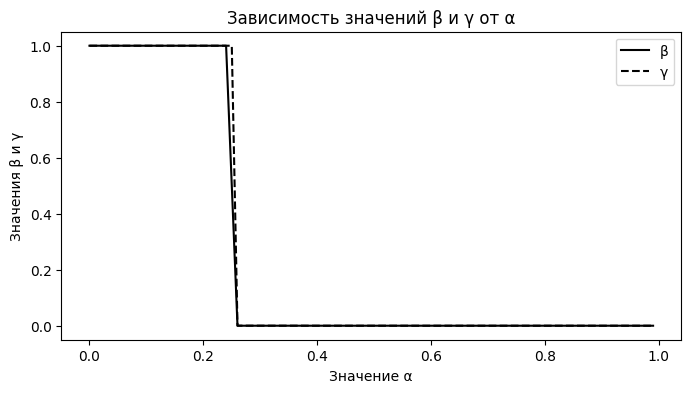
\includegraphics[width=0.8\linewidth]{inc/img/c3ex2alpha}
	\caption{График зависимости $ \beta$ и $ \gamma$ от $ \alpha$}
	\label{fig:c3ex2alpha}
\end{figure}

\begin{figure}[H]
	\centering
	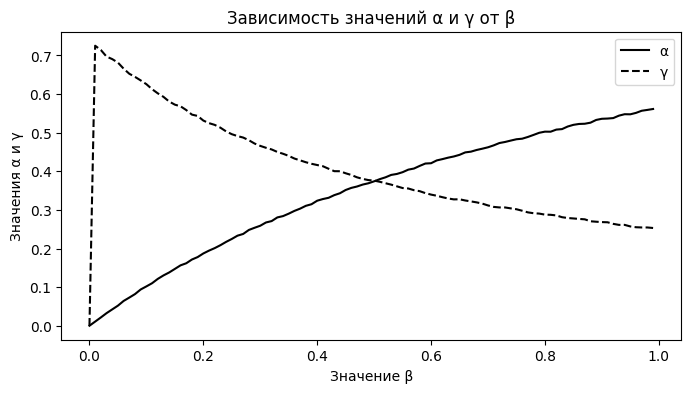
\includegraphics[width=0.8\linewidth]{inc/img/c3ex2beta}
	\caption{График зависимости $\alpha $ и $ \gamma$ от $ \beta$}
	\label{fig:c3ex2beta}
\end{figure}

\begin{figure}[H]
	\centering
	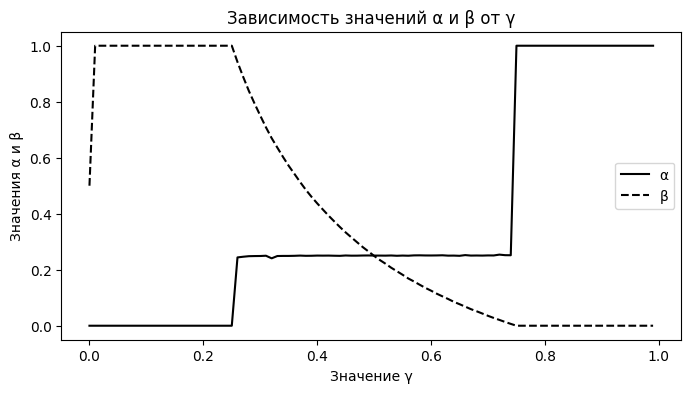
\includegraphics[width=0.8\linewidth]{inc/img/c3ex2gamma}
	\caption{График зависимости $\alpha $ и $ \beta$ от $ \gamma$}
	\label{fig:c3ex2gamma}
\end{figure}

\par
В соответствии с оценкой (\ref{eq:2.5}), вероятность проверки $\alpha$ влияет на решение чиновника о принятии взятки. В данном случае, критическое значение равно $0.25$, и на графиках \ref{fig:c3ex2alpha} и \ref{fig:c3ex2gamma} прослеживается изменение поведения участников при его преодолении инспектором.
\section{Второй пример. Модель коррупции в иерархической структуре}

В данной работе в качестве основного объекта исследования была выбрана игра «Иерархическая модель коррупции». 